% --- LaTeX Homework Template - S. Venkatraman ---

% --- Set document class and font size ---

\documentclass[letterpaper, 11pt]{article}

% --- Package imports ---

\usepackage{
  amsmath, amsthm, amssymb, mathtools, dsfont,	  % Math typesetting
  graphicx, wrapfig, subfig, float,                  % Figures and graphics formatting
  listings, color, inconsolata, pythonhighlight,     % Code formatting
  fancyhdr, sectsty, hyperref, enumerate, enumitem } % Headers/footers, section fonts, links, lists
  
  \usepackage{tikz}
  \usepackage{amsmath}
\usepackage{amsfonts}
  
  \tikzset{
  vtx/.style={circle, fill=black, inner sep=1.6pt},
  every picture/.style={>=latex}
}

\usetikzlibrary{positioning}

% --- Page layout settings ---

% Set page margins
\usepackage[left=0.7in, right=0.7in, bottom=1in, top=1.1in, headsep=0.2in]{geometry}
\usepackage{tikz}

% Anchor footnotes to the bottom of the page
\usepackage[bottom]{footmisc}



% Set line spacing
\renewcommand{\baselinestretch}{1.2}

% Set spacing between paragraphs
\setlength{\parskip}{1.5mm}

% Allow multi-line equations to break onto the next page
\allowdisplaybreaks

% Enumerated lists: make numbers flush left, with parentheses around them
\setlist[enumerate]{wide=0pt, leftmargin=21pt, labelwidth=0pt, align=left}
\setenumerate[1]{label={(\arabic*)}}

% --- Page formatting settings ---

% Set link colors for labeled items (blue) and citations (red)
\hypersetup{colorlinks=true, linkcolor=blue, citecolor=red}

% Make reference section title font smaller
\renewcommand{\refname}{\large\bf{References}}

% --- Settings for printing computer code ---

% Define colors for green text (comments), grey text (line numbers),
% and green frame around code
\definecolor{greenText}{rgb}{0.5, 0.7, 0.5}
\definecolor{greyText}{rgb}{0.5, 0.5, 0.5}
\definecolor{codeFrame}{rgb}{0.5, 0.7, 0.5}

% Define code settings
\lstdefinestyle{code} {
  frame=single, rulecolor=\color{codeFrame},            % Include a green frame around the code
  numbers=left,                                         % Include line numbers
  numbersep=8pt,                                        % Add space between line numbers and frame
  numberstyle=\tiny\color{greyText},                    % Line number font size (tiny) and color (grey)
  commentstyle=\color{greenText},                       % Put comments in green text
  basicstyle=\linespread{1.1}\ttfamily\footnotesize,    % Set code line spacing
  keywordstyle=\ttfamily\footnotesize,                  % No special formatting for keywords
  showstringspaces=false,                               % No marks for spaces
  xleftmargin=1.95em,                                   % Align code frame with main text
  framexleftmargin=1.6em,                               % Extend frame left margin to include line numbers
  breaklines=true,                                      % Wrap long lines of code
  postbreak=\mbox{\textcolor{greenText}{$\hookrightarrow$}\space} % Mark wrapped lines with an arrow
}

% Set all code listings to be styled with the above settings
\lstset{style=code}

% --- Math/Statistics commands ---

% Add a reference number to a single line of a multi-line equation
% Usage: "\numberthis\label{labelNameHere}" in an align or gather environment
\newcommand\numberthis{\addtocounter{equation}{1}\tag{\theequation}}

% Shortcut for bold text in math mode, e.g. $\b{X}$
\let\b\mathbf

% Shortcut for bold Greek letters, e.g. $\bg{\beta}$
\let\bg\boldsymbol

% Shortcut for calligraphic script, e.g. %\mc{M}$
\let\mc\mathcal

% \mathscr{(letter here)} is sometimes used to denote vector spaces
\usepackage[mathscr]{euscript}

% Convergence: right arrow with optional text on top
% E.g. $\converge[w]$ for weak convergence
\newcommand{\converge}[1][]{\xrightarrow{#1}}

% Normal distribution: arguments are the mean and variance
% E.g. $\normal{\mu}{\sigma}$
\newcommand{\normal}[2]{\mathcal{N}\left(#1,#2\right)}

% Uniform distribution: arguments are the left and right endpoints
% E.g. $\unif{0}{1}$
\newcommand{\unif}[2]{\text{Uniform}(#1,#2)}

% Independent and identically distributed random variables
% E.g. $ X_1,...,X_n \iid \normal{0}{1}$
\newcommand{\iid}{\stackrel{\smash{\text{iid}}}{\sim}}

% Equality: equals sign with optional text on top
% E.g. $X \equals[d] Y$ for equality in distribution
\newcommand{\equals}[1][]{\stackrel{\smash{#1}}{=}}

% Math mode symbols for common sets and spaces. Example usage: $\R$
\newcommand{\R}{\mathbb{R}}   % Real numbers
\newcommand{\C}{\mathbb{C}}   % Complex numbers
\newcommand{\Q}{\mathbb{Q}}   % Rational numbers
\newcommand{\Z}{\mathbb{Z}}   % Integers
\newcommand{\N}{\mathbb{N}}   % Natural numbers
\newcommand{\F}{\mathcal{F}}  % Calligraphic F for a sigma algebra
\newcommand{\El}{\mathcal{L}} % Calligraphic L, e.g. for L^p spaces

% Math mode symbols for probability
\newcommand{\pr}{\mathbb{P}}    % Probability measure
\newcommand{\E}{\mathbb{E}}     % Expectation, e.g. $\E(X)$
\newcommand{\var}{\text{Var}}   % Variance, e.g. $\var(X)$
\newcommand{\cov}{\text{Cov}}   % Covariance, e.g. $\cov(X,Y)$
\newcommand{\corr}{\text{Corr}} % Correlation, e.g. $\corr(X,Y)$
\newcommand{\B}{\mathcal{B}}    % Borel sigma-algebra

% Other miscellaneous symbols
\newcommand{\tth}{\text{th}}	% Non-italicized 'th', e.g. $n^\tth$
\newcommand{\Oh}{\mathcal{O}}	% Big-O notation, e.g. $\O(n)$
\newcommand{\1}{\mathds{1}}	% Indicator function, e.g. $\1_A$

% Additional commands for math mode
\DeclareMathOperator*{\argmax}{argmax}    % Argmax, e.g. $\argmax_{x\in[0,1]} f(x)$
\DeclareMathOperator*{\argmin}{argmin}    % Argmin, e.g. $\argmin_{x\in[0,1]} f(x)$
\DeclareMathOperator*{\spann}{Span}       % Span, e.g. $\spann\{X_1,...,X_n\}$
\DeclareMathOperator*{\bias}{Bias}        % Bias, e.g. $\bias(\hat\theta)$
\DeclareMathOperator*{\ran}{ran}          % Range of an operator, e.g. $\ran(T) 
\DeclareMathOperator*{\dv}{d\!}           % Non-italicized 'with respect to', e.g. $\int f(x) \dv x$
\DeclareMathOperator*{\diag}{diag}        % Diagonal of a matrix, e.g. $\diag(M)$
\DeclareMathOperator*{\trace}{trace}      % Trace of a matrix, e.g. $\trace(M)$

% Numbered theorem, lemma, etc. settings - e.g., a definition, lemma, and theorem appearing in that 
% order in Section 2 will be numbered Definition 2.1, Lemma 2.2, Theorem 2.3. 
% Example usage: \begin{theorem}[Name of theorem] Theorem statement \end{theorem}
\theoremstyle{definition}
\newtheorem{theorem}{Theorem}[section]
\newtheorem{proposition}[theorem]{Proposition}
\newtheorem{lemma}[theorem]{Lemma}
\newtheorem{corollary}[theorem]{Corollary}
\newtheorem{definition}[theorem]{Definition}
\newtheorem{example}[theorem]{Example}
\newtheorem{remark}[theorem]{Remark}

% Un-numbered theorem, lemma, etc. settings
% Example usage: \begin{lemma*}[Name of lemma] Lemma statement \end{lemma*}
\newtheorem*{theorem*}{Theorem}
\newtheorem*{proposition*}{Proposition}
\newtheorem*{lemma*}{Lemma}
\newtheorem*{corollary*}{Corollary}
\newtheorem*{definition*}{Definition}
\newtheorem*{example*}{Example}
\newtheorem*{remark*}{Remark}
\newtheorem*{claim}{Claim}
\newcommand{\Tau}{\mathcal{T}}
\newcommand{\PSet}{\mathcal{P}}





% --- Left/right header text (to appear on every page) ---

% Include a line underneath the header, no footer line
\pagestyle{fancy}
\renewcommand{\footrulewidth}{0pt}
\renewcommand{\headrulewidth}{0.4pt}

% Left header text: course name/assignment number
\lhead{MAM4000W, Graph Theory -- Chapter 5 Problems}

% Right header text: your name
\rhead{Alex Cristaudo, CRSALE010}

% --- Document starts here ---

\begin{document}

\subsection*{Question 1: Find $\chi (Q_t)$}
We will show that $Q_t$ is bipartite. Let $V_1$ be the set of binary strings with an odd number of 1's, and $V_2$ be the set of all binary strings with an even number of ones. Then, since in $Q_t$ two vertices are adjacent if and only if their binary strings differ by exactly one digit, we only have edges between vertices with different parity of ones digits. Changing one digit from 0 to 1 or 1 to 0 changes the number of ones by exactly one. Then it follows that $\chi (Q_t) = 2$.

\subsection*{Question 2: Determine the chromatic number of the Petersen Graph.}
\begin{figure}[h]
\centering
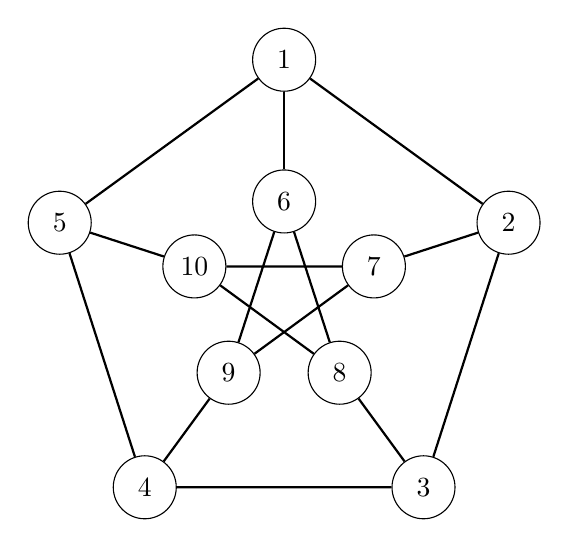
\begin{tikzpicture}[scale=1.5]
    % Outer pentagon vertices
    \node[circle, fill=white!30, draw, minimum size=8mm] (O1) at (0,2) {1};
    \node[circle, fill=white!30, draw, minimum size=8mm] (O2) at (1.9,0.62) {2};
    \node[circle, fill=white!30, draw, minimum size=8mm] (O3) at (1.18,-1.62) {3};
    \node[circle, fill=white!30, draw, minimum size=8mm] (O4) at (-1.18,-1.62) {4};
    \node[circle, fill=white!30, draw, minimum size=8mm] (O5) at (-1.9,0.62) {5};
    
    % Inner pentagram vertices
    \node[circle, fill=white!30, draw, minimum size=8mm] (I1) at (0,0.8) {6};
    \node[circle, fill=white!30, draw, minimum size=8mm] (I2) at (0.76,0.25) {7};
    \node[circle, fill=white!30, draw, minimum size=8mm] (I3) at (0.47,-0.65) {8};
    \node[circle, fill=white!30, draw, minimum size=8mm] (I4) at (-0.47,-0.65) {9};
    \node[circle, fill=white!30, draw, minimum size=8mm] (I5) at (-0.76,0.25) {10};
    
    % Outer pentagon edges
    \draw[thick] (O1) -- (O2) -- (O3) -- (O4) -- (O5) -- (O1);
    
    % Inner pentagram edges (connecting every other vertex)
    \draw[thick] (I1) -- (I3) -- (I5) -- (I2) -- (I4) -- (I1);
    
    % Spokes connecting outer to inner
    \draw[thick] (O1) -- (I1);
    \draw[thick] (O2) -- (I2);
    \draw[thick] (O3) -- (I3);
    \draw[thick] (O4) -- (I4);
    \draw[thick] (O5) -- (I5);
    
\end{tikzpicture}
\caption{The Petersen Graph}
\label{fig:petersen}
\end{figure}
~\\
The odd cycle implies that we need at least 3 colours to properly colour the Petersen Graph. Such a colouring is obtained via:
\begin{figure}[h]
\centering
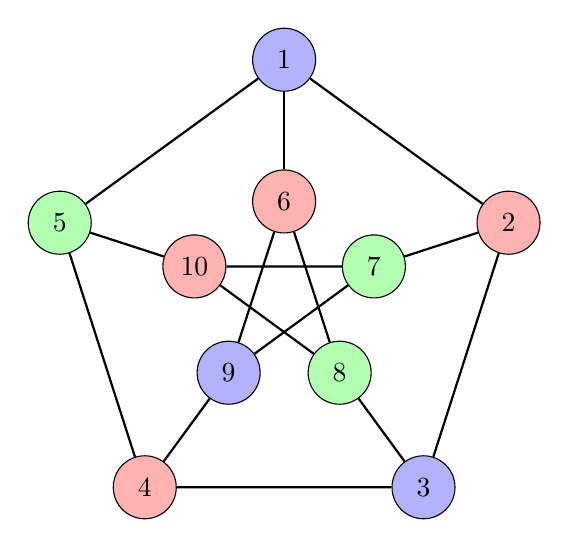
\begin{tikzpicture}[scale=1.5]
    % Outer pentagon vertices
    \node[circle, fill=blue!30, draw, minimum size=8mm] (O1) at (0,2) {1};
    \node[circle, fill=red!30, draw, minimum size=8mm] (O2) at (1.9,0.62) {2};
    \node[circle, fill=blue!30, draw, minimum size=8mm] (O3) at (1.18,-1.62) {3};
    \node[circle, fill=red!30, draw, minimum size=8mm] (O4) at (-1.18,-1.62) {4};
    \node[circle, fill=green!30, draw, minimum size=8mm] (O5) at (-1.9,0.62) {5};
    
    % Inner pentagram vertices
    \node[circle, fill=red!30, draw, minimum size=8mm] (I1) at (0,0.8) {6};
    \node[circle, fill=green!30, draw, minimum size=8mm] (I2) at (0.76,0.25) {7};
    \node[circle, fill=green!30, draw, minimum size=8mm] (I3) at (0.47,-0.65) {8};
    \node[circle, fill=blue!30, draw, minimum size=8mm] (I4) at (-0.47,-0.65) {9};
    \node[circle, fill=red!30, draw, minimum size=8mm] (I5) at (-0.76,0.25) {10};
    
    % Outer pentagon edges
    \draw[thick] (O1) -- (O2) -- (O3) -- (O4) -- (O5) -- (O1);
    
    % Inner pentagram edges (connecting every other vertex)
    \draw[thick] (I1) -- (I3) -- (I5) -- (I2) -- (I4) -- (I1);
    
    % Spokes connecting outer to inner
    \draw[thick] (O1) -- (I1);
    \draw[thick] (O2) -- (I2);
    \draw[thick] (O3) -- (I3);
    \draw[thick] (O4) -- (I4);
    \draw[thick] (O5) -- (I5);
    
\end{tikzpicture}
\caption{The Petersen Graph}
\label{fig:petersen}
\end{figure}
~\\
Thus $\chi (G) = 3$ for the Petersen Graph.


\subsection*{Question 3: Prove Theorem 5.2.3.}
(a) Suppose $G$ is $k$-chromatic and has a cut-vertex $v$. Then we can write $G = H \cup K$ for subgraphs $H$ and $K$ who only intersect at $v$. Then $\chi (G) = \max \{\chi (H), \chi (K)\}$. Without loss of generality, assume $\chi (H) = k$. Take any $u \in K$. Then $H \subseteq G - v$ so $\chi (G-v) = k$, a contradiction. ~\\ (b) Proceed the same as (a) and take some edge $e \in E(K)$, then $\chi (G- e ) = k$, a contradiction. ~\\ (c) We will prove the contrapositive. Suppose that $G$ is not critically $k$-chromatic, but is minimally $k$-chromatic. We must show $G$ has isolated vertices. Since $G$ is not critically $k$-chromatic, there is some vertex $v \in G$ such that $\chi (G-v) = k$. If $v$ is not isolated, it is incident to some edges. By removing all edges incident to $v$, we get a new graph $G'$ such that $\chi (G') \le k-1$ (removing any edge results in a graph with chromatic number $k-1$, removing further edges cannot increase the chromatic number). In this graph, $v$ is isolated so does not affect the chromatic number. So $\chi (G' - v) \le k-1$. But $G' - v = G-v$, giving us a contradiction. So $v$ has no incident edges and is isolated.

\subsection*{Question 4: If $G$ is critically $2$-chromatic, or if $G$ is minimally $2$-chromatic and has no isolated
vertices, prove that $G \cong K_2$}
First notice that if $G$ has no isolated vertices and is minimally $2$-chromatic, then it is critically $2$-chromatic, so we simply consider the case when $G$ is critically $2$-chromatic. Since $G$ is $2$-chromatic, it is bipartite. Let $V_1$ and $V_2$ be the partite sets. If $|V_1| > 1$ or $|V_2| > 1$, then taking any element $u$ in the set with size greater than 1, the graph $G - v$ requires 2 colours to properly colour (as it is bipartite). Thus $|V_1| = |V_2| = 1$, and we simply have 2 vertices connected by an edge. So $G \cong K_2$. (Otherwise, clearly $G$ contains $K_2$ as a subgraph. If it is not $K_2$ itself, it clearly has a vertex it can remove and it is still 2-chromatic)

\subsection*{Question 5: If $G$ is critically 3-chromatic, or if $G$ is minimally 3-chromatic and has no isolated
vertices, prove that $G$ is an odd cycle}
First notice that if $G$ has no isolated vertices and is minimally $3$-chromatic, then it is critically $3$-chromatic, so we simply consider the case when $G$ is critically $3$-chromatic. Since $G$ is not 2-chromatic, it is not bipartite. Thus it contains an odd cycle. If $G$ itself is the odd cycle, we are done. Otherwise $G$ has a vertex $v$ not in the cycle. Thus $G-v$ contains this odd cycle and must be 3-chromatic, a contradiction.


\subsection*{Question 6: Prove that a nontrivial graph $G$ is $k$-edge-connected if and only if there exists no
nonempty proper subset $W$ of $V(G)$ such that the number of edges between $W$ and
$V(G) - W$ is less than $k$.}

Suppose $G$ is $k$-edge-connected and let $W \subseteq V(G)$ be a proper subset, and $E(G[W])$ be the edges between $W$ and $V(G) - W$. Notice that $G - E(G[W])$ is is disconnected, if $W \ne \emptyset$ or $W \ne V(G)$ (which is given since it is a proper subset). So $|E(G[W])| \ge k$, as $G$ is $k$-edge-connected. 
Now suppose that there is no nonempty proper subset $W$ of $V(G)$ such that the number of edges between $W$ and $V(G) - W$ is less than $k$. Let $M$ be an minimal edge-cut of $G$. Then, $G$ is split into two components $C_1$ and $C_2$. Take $W = C_1$, then $V(G) - W = C_2$, and the edges between $C_1$ and $C_2$ is $M$. So $|M| \ge k$ so $G$ is $k$-edge-connected.

\subsection*{Question 7: Determine $\chi (C_3 \times C_3)$. Hence prove that $C_3 \times C_3$ is perfect.}

\begin{center}
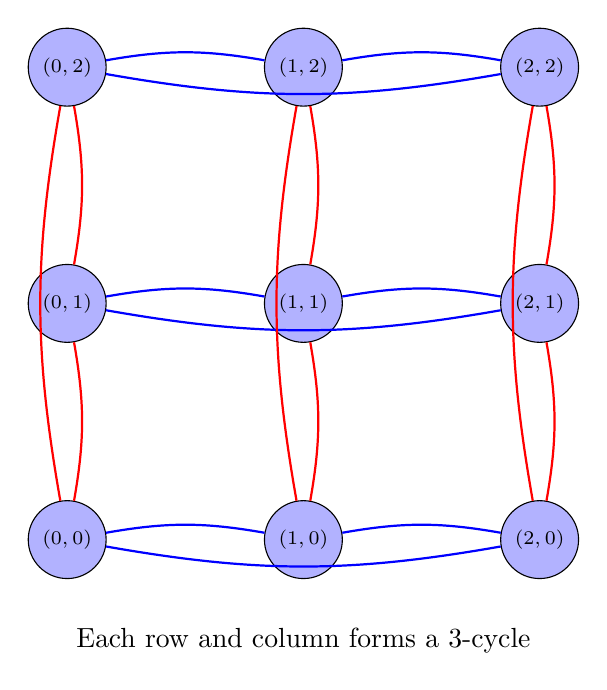
\begin{tikzpicture}[scale=2]
    % Grid positions
    \foreach \i in {0,1,2}
        \foreach \j in {0,1,2}
            \node[circle, draw, fill=blue!30, minimum size=8mm, font=\scriptsize] (v\i\j) at (\i*1.5, \j*1.5) {$(\i,\j)$};
    
    % All edges showing the cyclic nature clearly
    % Horizontal 3-cycles
    \foreach \j in {0,1,2} {
        \draw[thick, blue] (v0\j) to[bend left=10] (v1\j);
        \draw[thick, blue] (v1\j) to[bend left=10] (v2\j);
        \draw[thick, blue] (v2\j) to[bend left=10] (v0\j);
    }
    
    % Vertical 3-cycles  
    \foreach \i in {0,1,2} {
        \draw[thick, red] (v\i 0) to[bend right=10] (v\i 1);
        \draw[thick, red] (v\i 1) to[bend right=10] (v\i 2);
        \draw[thick, red] (v\i 2) to[bend right=10] (v\i 0);
    }
    
    \node[below] at (1.5, -0.5) {Each row and column forms a 3-cycle};
\end{tikzpicture}
\end{center}
Since this graph contains $C_3$, at least 3 colours are needed. We get a proper 3-colouring by using the colouring:
\[
1 \ \ 2 \ \ 3
\]\[
2 \ \ 3 \ \ 1
\]\[
3 \ \ 1 \ \ 2
\]
where no column and row has the same colour twice. Clearly $\omega (C_3 \times C_3) = 3$. Let $H$ be an induced subgraph of $C_3 \times C_3$. If $H$ contains $C_3$ as a subgraph, then clearly $\chi (H) = \omega (H) = 3$ (where $\chi (H) \le 3$ as a subgraph, but needs 3 colours as it contains $C_3$). If $H$ contains $K_2$ as its largest complete subgraph, then at least one vertex from every row and column has to be removed. We may assume, up to isomorphism, that $H$ is contained in:
\begin{center}
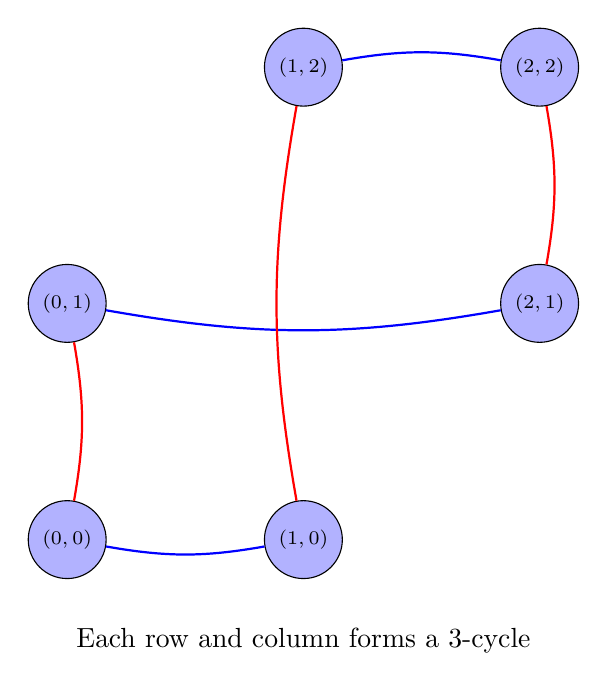
\begin{tikzpicture}[scale=2]
    % Grid positions
    \foreach \i in {1}
        \foreach \j in {0,2}
            \node[circle, draw, fill=blue!30, minimum size=8mm, font=\scriptsize] (v\i\j) at (\i*1.5, \j*1.5) {$(\i,\j)$};

    \foreach \i in {2}
        \foreach \j in {1,2}
            \node[circle, draw, fill=blue!30, minimum size=8mm, font=\scriptsize] (v\i\j) at (\i*1.5, \j*1.5) {$(\i,\j)$};
            
    \foreach \i in {0}
        \foreach \j in {0,1}
            \node[circle, draw, fill=blue!30, minimum size=8mm, font=\scriptsize] (v\i\j) at (\i*1.5, \j*1.5) {$(\i,\j)$};  
    
    % All edges showing the cyclic nature clearly
    % Horizontal 3-cycles
    \foreach \j in {0} {
        \draw[thick, blue] (v1\j) to[bend left=10] (v0\j);
    }
    
      \foreach \j in {1} {

        \draw[thick, blue] (v2\j) to[bend left=10] (v0\j);
    }
    
    \foreach \j in {2} {
        \draw[thick, blue] (v1\j) to[bend left=10] (v2\j);
    }
    
    % Vertical 3-cycles  
    \foreach \i in {1} {

        \draw[thick, red] (v\i 2) to[bend right=10] (v\i 0);
    }
     \foreach \i in {2} {

        \draw[thick, red] (v\i 1) to[bend right=10] (v\i 2);

    }
    
    \foreach \i in {0} {
        \draw[thick, red] (v\i 0) to[bend right=10] (v\i 1);
    }
    
    \node[below] at (1.5, -0.5) {Each row and column forms a 3-cycle};
\end{tikzpicture}
\end{center}
~\\Which is $C_6$ and thus $\chi (H) = 2$. The case when $\omega (H) = 1$ is the trivial graph so $\chi (H) = 1$ as well. So $C_3 \times C_3$ is perfect. ~\\~\\If we use the equivalent formulation, we need to show $C_3 \times C_3$ and $\overline{C_3 \times C_3}$ contains no induced odd cycles of length at least 5. In order to have an induced odd cycle, we must use an edge jumping over another. We also cannot have all 3 columns, we must remove one entirely. We must also remove the middle vertex in each row and column (otherwise we end up with an instance of $K_3$ and that cannot be an odd cycle attached to other vertices). But then we are left with $C_4$, which is not odd. In $\overline{C_3 \times C_3}$, we use the same reasoning to remove the middle vertex (removes the instance of $K_3$). Then have isolated vertices in the corners that we must remove, then are left with $C_4$. So $C_3 \times C_3$ is perfect.

\subsection*{Question 8: If $a$ and $b$ are positive numbers, prove that $\sqrt{ab} \le \frac{a+b}{2}$}.
We know that $(\sqrt{a}-\sqrt{b})^2 \ge 0$. Expanding, we get \[
a + b - 2\sqrt{ab} \ge 0 \iff \sqrt{ab} \le \frac{a+b}{2}
\]
as required.

\subsection*{Question 9: Prove Theorem 5.3.2.}
Let $M = \max \{\delta (H): H \text{ is an induced subgraph of } G\}$
We will index the vertices in $G$ as follows:\\ Let $v_1$ be the vertex of minimal degree in $G_1 := G$. Define $G_2 := G - v_1$. Let $v_k$ be the vertex of minimal degree in $G_{k}$ and $G_{k+1} := G_{k} - v_k$. Then $\delta (G_k) = \deg _{G_{k}}v_{k} \le M$. We then perform the Greedy Algorithm in this selection in reverse order. Let $v_n$ be coloured 1, and continue. Then, at some point $v_k$, the neighbours of $v_k$ that have already been coloured are in $G_k$. But $\deg _{G_k} v_k = \delta (G_k) \le M$. So we can always find a colour in $\{1,2,...,M+1\}$ to colour $v_k$. So $\chi (G) \le M+1$.
\subsection*{Question 10: Let $G$ be a graph of order $n$. A set $S \subseteq V(G)$ is said to be independent if no two
vertices of $S$ are adjacent. The independence number of $G$ is $\beta(G) = \max\{|S|: S \text{ is an independent set of vertices}\}$. Prove that $n/\beta (G) \le \chi (G) \le n+1-\beta (G)$}
Let $S$ be a maximal independent set. We can colour every vertex in $S$ with one colour. Then, there are $n - \beta (G)$ vertices uncoloured. We can colour every other vertex with a unique colour to give a proper colouring with a total of $n+1 - \beta (G)$ vertices. Thus $\kappa (G) \le n+1 - \beta (G)$. Consider colouring $G$ with a proper $\chi (G)$-colouring and consider the colour classes $C_1,C_2,...,C_{\chi (G)}$. Clearly $|C_i| \le \beta (G)$ for all $1 \le i \le \beta (G)$. So \[
n = \sum \limits _{i=1}^{\chi (G)} |C_i| \le \chi (G) \beta (G) \text{ so }\chi(G) \ge n/\beta (G)
\]


\subsection*{Question 11: Prove that for every pair $k, \ell$ of integers with $k \ge \ell \ge 3$, there exists a graph $G$ with
$\chi (G) = k$ and $\omega (G) = \ell$}
By Theorem 5.4.3, there is a triangle-free graph $G$ with $\chi (G) = k$. We simply modify $G$ by taking any vertex $v \in V(G)$ and attaching it to a copy of $K_{\ell}$. We clearly colour the $K_\ell$ subgraph with a proper $\ell$-colouring. Call this graph $H$. Then $\ell \le k$. $\chi (H) = k$. Since $\omega(G)=2$, clearly $\omega(H) = \ell$ as required. 
(see notes for Mycielski's construction to increase the chromatic number, while keeping the clique number the same).


\subsection*{Question 12: Prove that every graph of order $6$ with chromatic number $3$ has at most $12$ edges.}
Colour graph $G$ with a $3$-colouring, and let $x,y,z$ be the number of vertices coloured $1,2,3$ respectively. Then $x+y+z=6$. In $G$, vertices can only be adjacent if they are differently coloured, so the maximum number of edges is given by $xy + yz + xz$. But \[
36 = (x+y+z)^2 = x^2+y^2+z^2 + 2(xy+yz+xz)
\]
And $x,y,z\ge 1$. If, without loss of generality, $z=1$, then, without loss of generality, $x \ge 3$. If \begin{align*}
(x,y,z) & = (3,2,1) \Rightarrow x^2 + y^2 + z^2 = 14 \\ 
(x,y,z) & = (4,1,1) \Rightarrow x^2 + y^2 + z^2 = 18 
\end{align*}
If every $x,y,z \ge 2$, then $x=y=z=2$ and $x^2+y^2+z^2 = 12$. Thus we conclude $x^2+y^2+z^2 \ge 12$ and so \[
m \le xy + yz + xz = (36 - x^2+y^2+z^2)/2 \le 12
\]
as required.

\subsection*{Question 13: Prove that in every $r$-regular graph $G$ of order $n$, we must have $\chi (G) \ge n/(n-r)$}
Colour $G$ with a $\chi(G)$-colouring and consider the colour classes $C_1,C_2,...,C_{\chi(G)}$. Any vertex in a specific colour class has exactly $r$ neighbours, and every colour class is nonempty (otherwise it contradicts our $\chi (G)$ chromatic number), so a specific colour class has at most $n-r$ elements. Then \[
n = \sum \limits _{i=1}^{\chi (G)} |C_i| \le \chi (G) (n-r)
\]
as required.

\subsection*{Question 14: Let $n$ be odd. Prove that $C_n + C_n$ is $6$-critical}
By colouring each $C_n$ instance with 3 colours (different for the different subgraphs), we get a proper $6$-colouring. So $\chi (C_n + C_n) \le 6$. On the other hand, let $H_1$ and $H_2$ denote the $C_n$ instances. $H_1$ and $H_2$ require at least 3 colours to properly colour them, and since every vertex in $H_1$ is incident to every vertex in $H_2$, these two subgraphs cannot share a colour. Thus we need at least 6 colours. Thus $\chi (C_n + C_n) = 6$. Let $v \in V(C_n + C_n)$. Then $G - v \cong C_n + P_{n-1}$. Again, we need at least 3 colours to colour $C_n$, and at least $2$ to colour $P_{n-1}$, and in $C_n + P_{n-1}$, these subgraphs cannot share a colour so we need at least 5 colours. Colouring with 5 is possible by colouring $C_n$ with colours $\{1,2,3\}$ (as usual), and $P_{n-1}$ with $\{4,5\}$ (as usual). So $\chi (G - v) = 5$ and $C_n + C_n$ is $6$-critical.

\subsection*{Question 15: A latin square is an $n \times n$ matrix in which each of the numbers $1$ to $n$ appear exactly once in each row and exactly once in each column. Recast the problem of constructing a Latin square as a graph colouring problem.}
(See Question 7 for a visual idea) Our latin square can be represented as the graph $K_{n} \times K_n$, where edges are between vertices 'in the same row or column'. Then the problem of constructing a Latin square becomes a problem of finding a proper $n$-colouring of $K_n \times K_n$.

\subsection*{Question 16: Prove or disprove: If $G_1$ and $G_2$ are class one graphs and $H$ is a graph with $G_1 \subseteq H \subseteq G_2$, then $H$ is of class one.}
No. Consider $G_1 = K_2$, $H = K_3$ and $G_2 = K_4$
\subsection*{Question 17: Show that a cubic graph with a bridge has edge chromatic number 4.}
By Vizing's Theorem, we know $3 \le \chi ' (G) \le 4$. We must show that $\chi ' (G) = 3$ is not possible. Assume otherwise and that we have a proper $3$-edge-colouring. Since $G$ is 3-regular, every vertex is adjacent to all three colours. Without loss of generality, assume the bridge is coloured $1$. Let $C_1, C_2, C_3$ be the colour classes in $G$ and consider the subgraph $G[C_1 \cup C_2]$. This is then 2-regular (possibly disconnected). Let $C$ be the component containing the bridge. Being 2-regular means it contains an Eulerian circuit and thus a cycle, contradicting that we have a bridge. Thus $\kappa ' (G) = 4$.

\subsection*{Question 17: Show that every non-empty regular graph of odd order is of class two.}
Suppose that $G$ is an $r$-regular graph of odd order. Suppose, to the contrary, that $\chi ' (G) = r$. Every vertex has exactly $r$ neighbours, so every vertex has an edge of every colour. Each edge has 2 vertices, so, if $n = 2k + 1$ for some $k \in \mathbb{Z}$, we have at most $\lfloor (2k + 1)/2 \rfloor = k$ instances of one colour (accounting for double counting). If we have an $r$-colouring, we have at most $rk$ colours. But, by the Handshaking Lemma, \[
2m = \sum \limits _{v \in V} \deg v = nr \iff m = kr + \frac{r}{2} > kr
\] 
So we cannot find an edge $r$-colouring and thus $G$ is in class two.

\subsection*{Question 18: $X''(G)$ is defined as the minimum number of colours required to colour vertices and
edges of G such that no two incident or adjacent elements have the same colour. The Total Colouring Conjecture conjectures that $X''(G) \le 2 + \Delta (G)$.}
\subsection*{\ \ (a) Prove that $X''(G) \ge 1 + \Delta (G)$ for every graph $G$.}
To colour the edges properly, we need at least $\Delta (G)$ colours ($\chi ' (G) \ge \Delta (G)$). Now, consider the vertex $v$ with $\deg v = \Delta (G)$. All the edges incident to this vertex must use colours $\{1,2,..., \Delta (G)\}$, so we need at least one further colour to colour $G$. So $X''(G) \ge \Delta (G) + 1$.

\subsection*{\ \ (b) Verify the Total Colouring Conjecture for graphs $G$ with $\Delta (G) \le 2$}
We can simply consider connected graphs, as disconnected graphs will follow with each component satisfying the inequality and $\Delta (G) = \max \Delta (C_i), X''(G) = \max X''(C_i)$. So let $G$ be connected. If $\Delta (G) = 0$, $G$ is trivial graph and $X''(G) = 1$. If $\Delta (G) = 1$, then $G \cong K_2$ and $K''(G) = 3$. So let $\Delta (G) = 2$. Then $G$ is a union of paths and cycles. If we can show each of those satisfy the Total Colouring Conjecture, then so will $G$ by applying that colouring to each aspect (with possibly relabelling colours if needed)
\begin{itemize}
\item A path clearly needs 3 colours
\item An odd cycle needs 4 colours
\item An even cycle needs 3 colours
\end{itemize}
In all cases, we need less than or equal to $\Delta (G) + 2 = 4$ colours.

\subsection*{\ \ (c) Verify the Total Colouring Conjecture for bipartite graphs.}
We know that $X''(G) \le \chi (G) + \chi '(G)$, and that in a bipartite graph, $\chi (G) = 2$. If we use that a bipartite graph is class one, then we have our result (but it is a mission to prove). 
\end{document}